\documentclass[12pt]{article}

\usepackage[utf8]{inputenc}
\usepackage[T2A]{fontenc}
\usepackage[english,russian]{babel}
\usepackage{amssymb}
\usepackage{graphicx}
\graphicspath{ {images/} }

\textwidth=431pt
\textheight=600pt
\hoffset=-15pt
\voffset=-15pt

\usepackage{graphicx}
\usepackage{amsmath}
\makeatletter
\renewcommand{\@oddhead}{%
\vbox{%
\hbox to \textwidth{\strut \textit{Introduction to robotics, Final Project, Markeeva Larisa, Usvyatsov Mikhail} \hfill }
%\hbox to\textwidth{Лист\hfill Страница~\arabic{page}~из 2}
\hrule
\vspace{12pt}
}}
\renewcommand{\@oddfoot}{}
\makeatother

\begin{document}

%\tableofcontents

%\newpage

\begin{center}
\textbf{Final Project}
\end{center}

It was decided to build simplified model of human leg. The problem was that non simplified leg has 7 DoF, but it is very hard to compute IK in this situation, so one redundant DoF was deleted.

\bigskip
\bigskip
\bigskip 

\begin{center}
  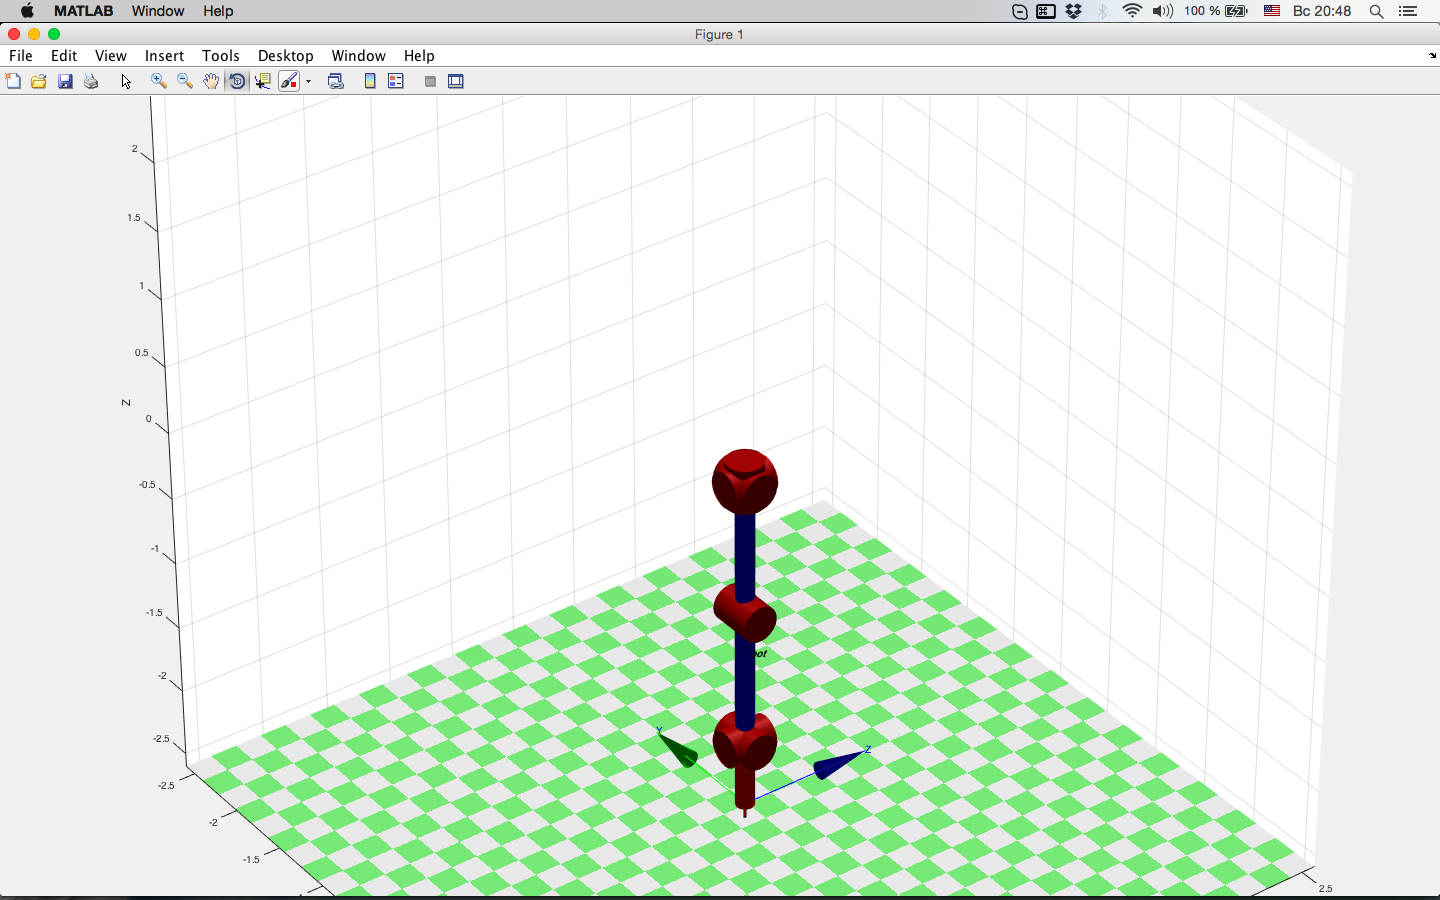
\includegraphics[width=15cm]{main}
\end{center}

DH:
\\
\begin{tabular}{|c|c|c|c|c|}
\hline
 & $a_{i-1}$ & $\alpha_{i-1}$ & $d_i$ & $\theta_i$ \\
 \hline
 1 & 0 & 0 & 0 & $\theta_1$\\
 2 & 0 & $\dfrac{\pi}{2}$ & 0 & $\theta2 - \dfrac{\pi}{2}$\\
 3 & 0 & $-\dfrac{\pi}{2}$ & 0 & $\theta3 + \pi$\\
 4 & $L_1$  & 0 & 0 & $\theta4$\\
 5 & $L_2$ & 0 & 0 & $\theta5 + \dfrac{\pi}{2}$\\
 6 & 0 & $-\dfrac{\pi}{2}$ & 0 & $\theta6$\\
 7 & $L_3$ & 0 & 0 & 0\\ 
\hline
\end{tabular}

\bigskip

Transformation matrices

\[^0_{1}T=\left[
\begin{array}{cccc}
cos(\theta_1) & -sin(\theta_1) & 0 & 0 \\
sin(\theta_1) & cos(\theta_1) & 0 & 0 \\
0 & 0 & 1 & 0\\
0 & 0 & 0 & 1
\end{array} \right]\]
\ 
\[^1_{2}T=\left[
\begin{array}{cccc}
cos(\theta_2 - \dfrac{\pi}{2}) & -sin(\theta_2 - \dfrac{\pi}{2}) & 0 & 0 \\
0 & 0 & -1 & 0\\
sin(\theta_2 - \dfrac{\pi}{2}) & cos(\theta_2 - \dfrac{\pi}{2}) & 0 & 0 \\
0 & 0 & 0 & 1
\end{array} \right]\]
\ 
\[^2_{3}T=\left[
\begin{array}{cccc}
cos(\theta_3 + \pi) & -sin(\theta_3 + \pi) & 0 & 0 \\
0 & 0 & 1 & 0\\
-sin(\theta_3 + \pi) & -cos(\theta_3 + \pi) & 0 & 0 \\
0 & 0 & 0 & 1
\end{array} \right]\]
\ 
\[^3_{4}T=\left[
\begin{array}{cccc}
cos(\theta_4) & -sin(\theta_4) & 0 & L_1 \\
sin(\theta_4) & cos(\theta_4) & 0 & 0 \\
0 & 0 & 1 & 0\\
0 & 0 & 0 & 1
\end{array} \right]\]
\
\[^4_{5}T=\left[
\begin{array}{cccc}
cos(\theta_5 + \dfrac{\pi}{2}) & -sin(\theta_5 + \dfrac{\pi}{2}) & 0 & L_2 \\
sin(\theta_5 + \dfrac{\pi}{2}) & cos(\theta_5 + \dfrac{\pi}{2}) & 0 & 0 \\
0 & 0 & 1 & 0\\
0 & 0 & 0 & 1
\end{array} \right]\]
\
\[^5_{6}T=\left[
\begin{array}{cccc}
cos(\theta_6) & -sin(\theta_6) & 0 & L_1 \\
0 & 0 & 1 & 0\\
- sin(\theta_6) & -cos(\theta_6) & 0 & 0 \\
0 & 0 & 0 & 1
\end{array} \right]\]
\
\[^6_{EE}T=\left[
\begin{array}{cccc}
1 & 0 & 0 & L_3 \\
0 & 1 & 0 & 0 \\
0 & 0 & 1 & 0\\
0 & 0 & 0 & 1
\end{array} \right]\]

$^0_{EE}T = ^0_{1}T ^1_{2}T ^2_{3}T ^3_{4}T ^4_{5}T ^5_{6}T ^6_{EE}T$

\bigskip 

First of all when we talk about IK problem, we should understand that we have not only position but also the orientation of the EE. For simplicity in this work as orientation will be used pitch roll and yaw.

Then we can calculate the coordinates of the heel:

$$
	\left\{
	\begin{array}{l l}
		H_x = x - L_3 sin(yaw) cos(pitch) &\\
		H_y = y - L_3 cos(yaw) cos(pitch) &\\
		H_z = z - L_3 sin(pitch) & 
	\end{array}
	\right.
$$

We can see that our simplification - deleting one DoF at foot helped us because roll will now definitely  cause the place of the knee due to the fact that this DoF can be guaranteed only by the hip.

Now we have enough information to compute angle $\theta_4$

$theta_4 = arccos \left( \dfrac{H^2_x + H^2_y + H^2_z) - L_1 - L_2}{2 L_1 L_2} \right)$

Now we can compute the point of intersection the knee and hip-heel. We we call this point Under Knee.

UK:

First of all we can find $\eta$ that is the coefficient that show how the point of UK derives the line from hip to the heel.

And after that it is obvious that UK = ($\eta H_x, \eta H_y, \eta H_z$)

After that we can find angles $\alpha$ and $\beta$ from the following: 

$$
	\left\{
	\begin{array}{l l}
		UK_x = L^{'}_1 sin(\alpha) cos(\beta) &\\
		UK_y = L^{'}_1 cos(\alpha) cos(\beta) &\\
		UK_z = L^{'}_1 sin(\beta) & 
	\end{array}
	\right.
$$

And so we are moving forward to compute the coordinates of the knee. We can calculate $K_0$ that shows coordinates of the knee when roll is equal to zero.

$$
	\left\{
	\begin{array}{l l}
		K0_x = h sin(\alpha) sin(\beta) + UK_x &\\
		K0_y = h sin(\beta) sin(\alpha) + UK_y &\\
		K0_z = h sin(\beta) + UK_z& 
	\end{array}
	\right.
$$

Where h is the distance between the knee and UK point.

And so we have find
$\theta_1 = roll$

$\theta_2 = \alpha$

$\theta_3 = \beta$

To find other two angles we will find the rotation around axes hip - heel and then after multiplying this rotation matrix by coordinates of vector $K_0$ we will find coordinates of point K - the knee. 

$\theta_5$ can be easily find from cosine theorem. And it is equal to arccos $\left(  \dfrac{L^2_2 + L^2_3 - Length_of_shin^2}{2 L_2 L_3} \right)$

After that it is not a big deal to find $\theta_6$ as yaw + $\nu$, where $\nu$ can be fined from $\nu = \dfrac{K_x - H_x}{sin(\alpha) \sqrt{K^2_x + K^2_y + K^2_z}}$

And now all the IK is solved.

\newpage

\begin{center}
\textbf{Appendix 1}
\end{center}

Implemented commands.

project - draw the robot, returns nothing

\begin{center}
  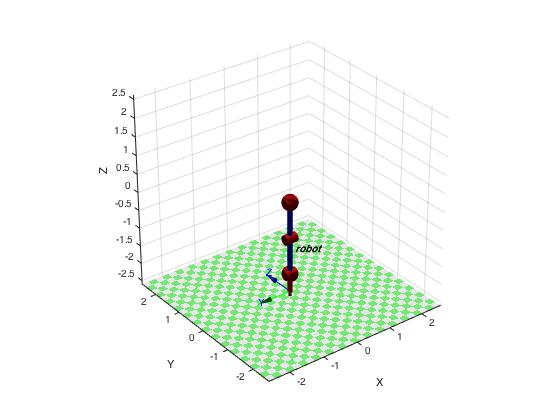
\includegraphics[width=15cm]{conf}
\end{center}

WHERE - returns the coordinates of EE and plots the configuration of the robot. Returns matrix 4*4 with position and orientation of EE.

\begin{center}
  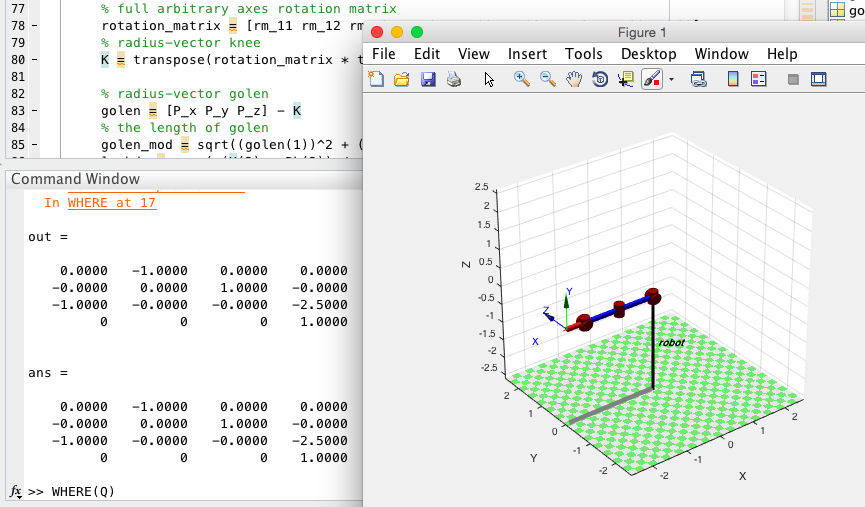
\includegraphics[width=15cm]{where}
\end{center}

WS\_DISPLAY - calculates reachable work space. Works long time. returns nothing. 

\begin{center}
  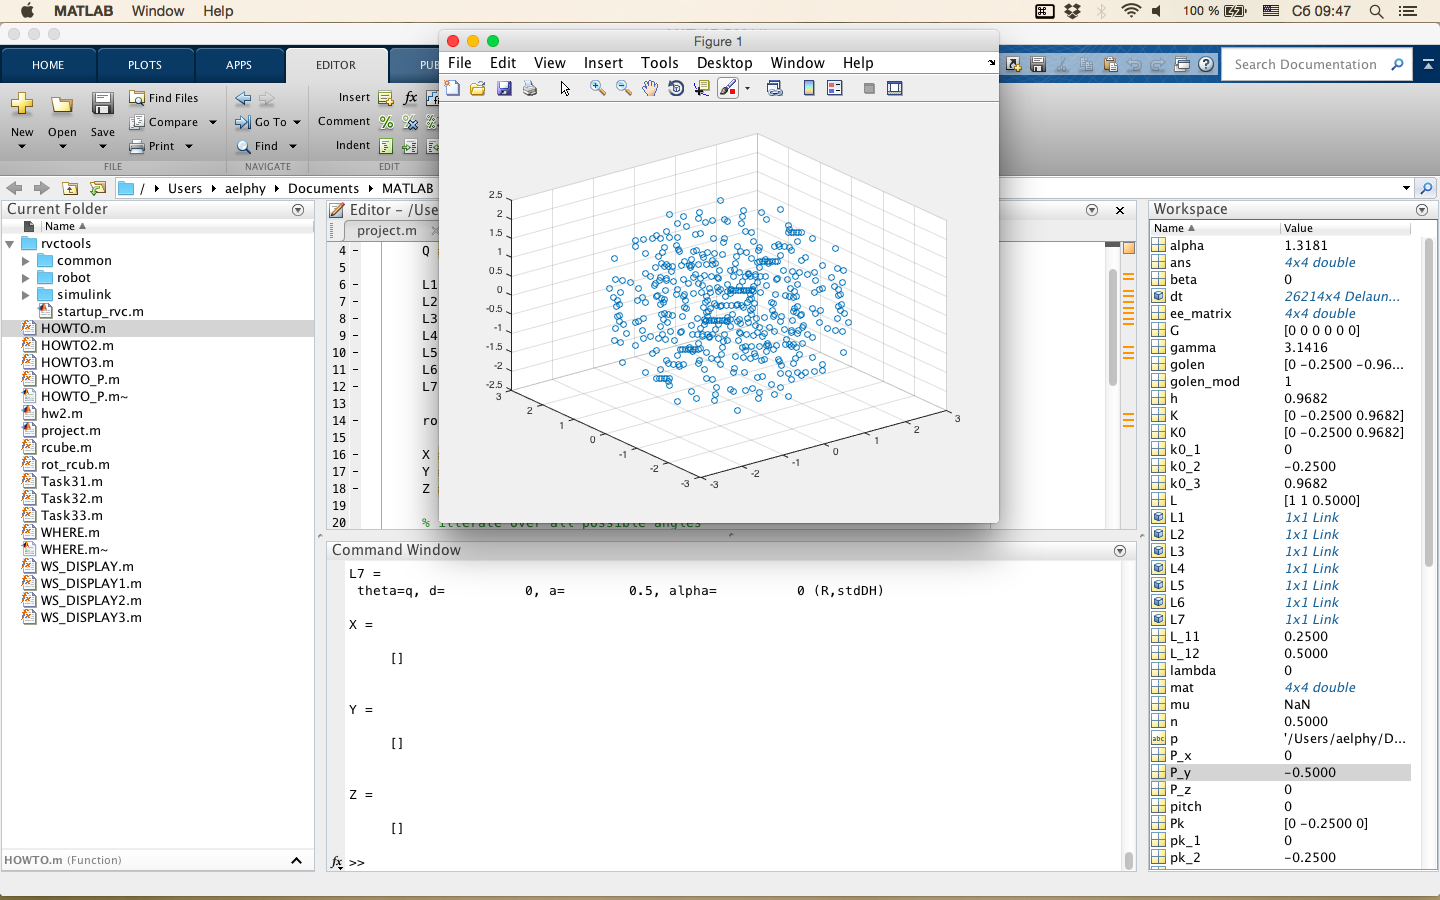
\includegraphics[width=15cm]{ws}
\end{center}

\newpage

HOWTO\_P - as input 4*4 matrix of position and orientation is needed. Solves the IK. Returns the 1*6 array of joint angles.

\begin{center}
  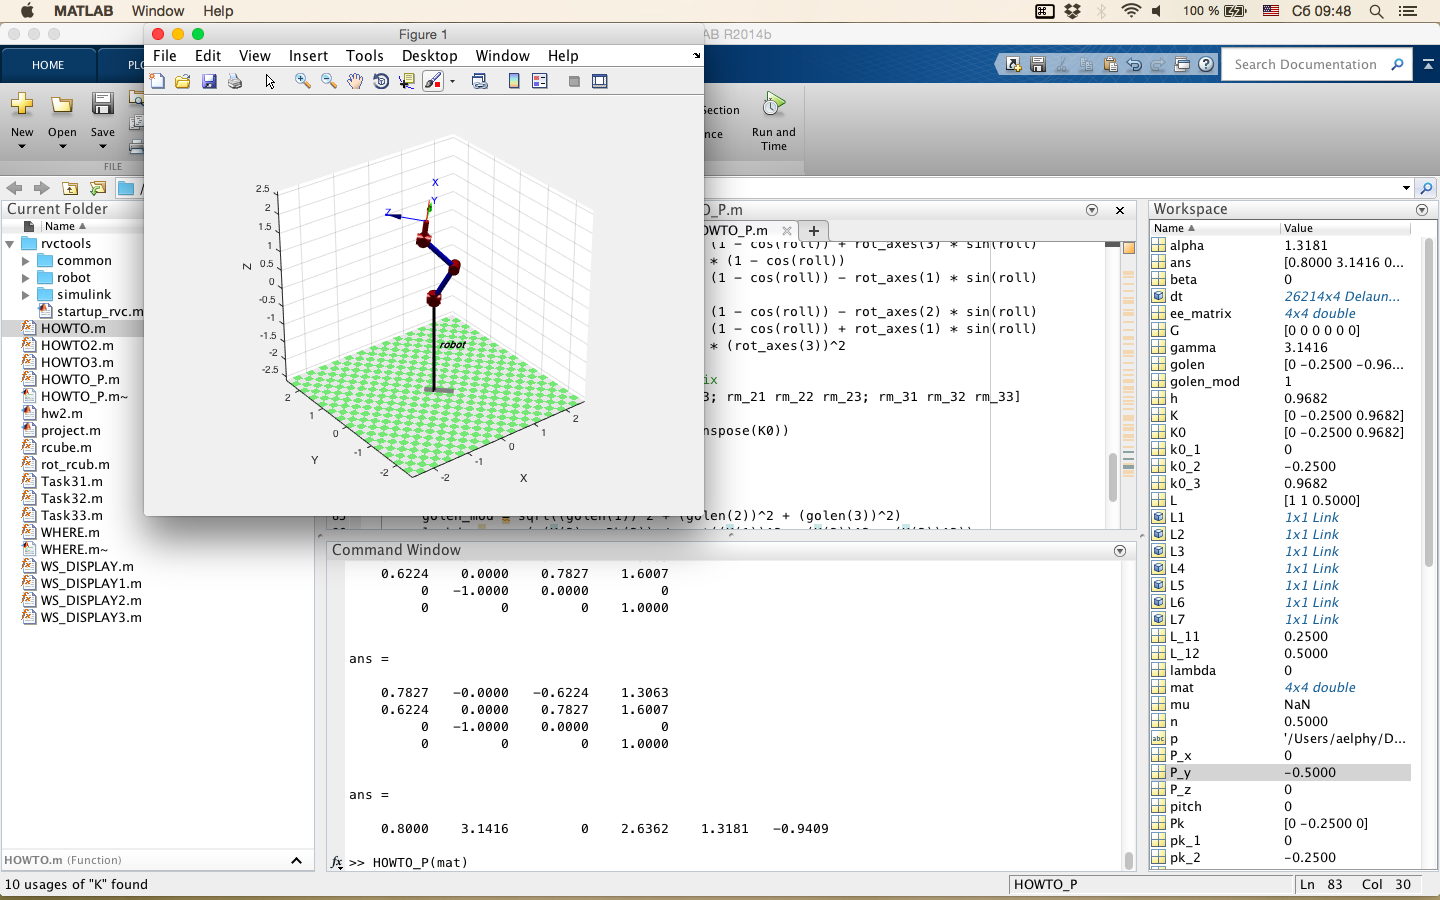
\includegraphics[width=15cm]{ht}
\end{center}

J23D - as input joint velocities vector 1*6. 

\begin{center}
  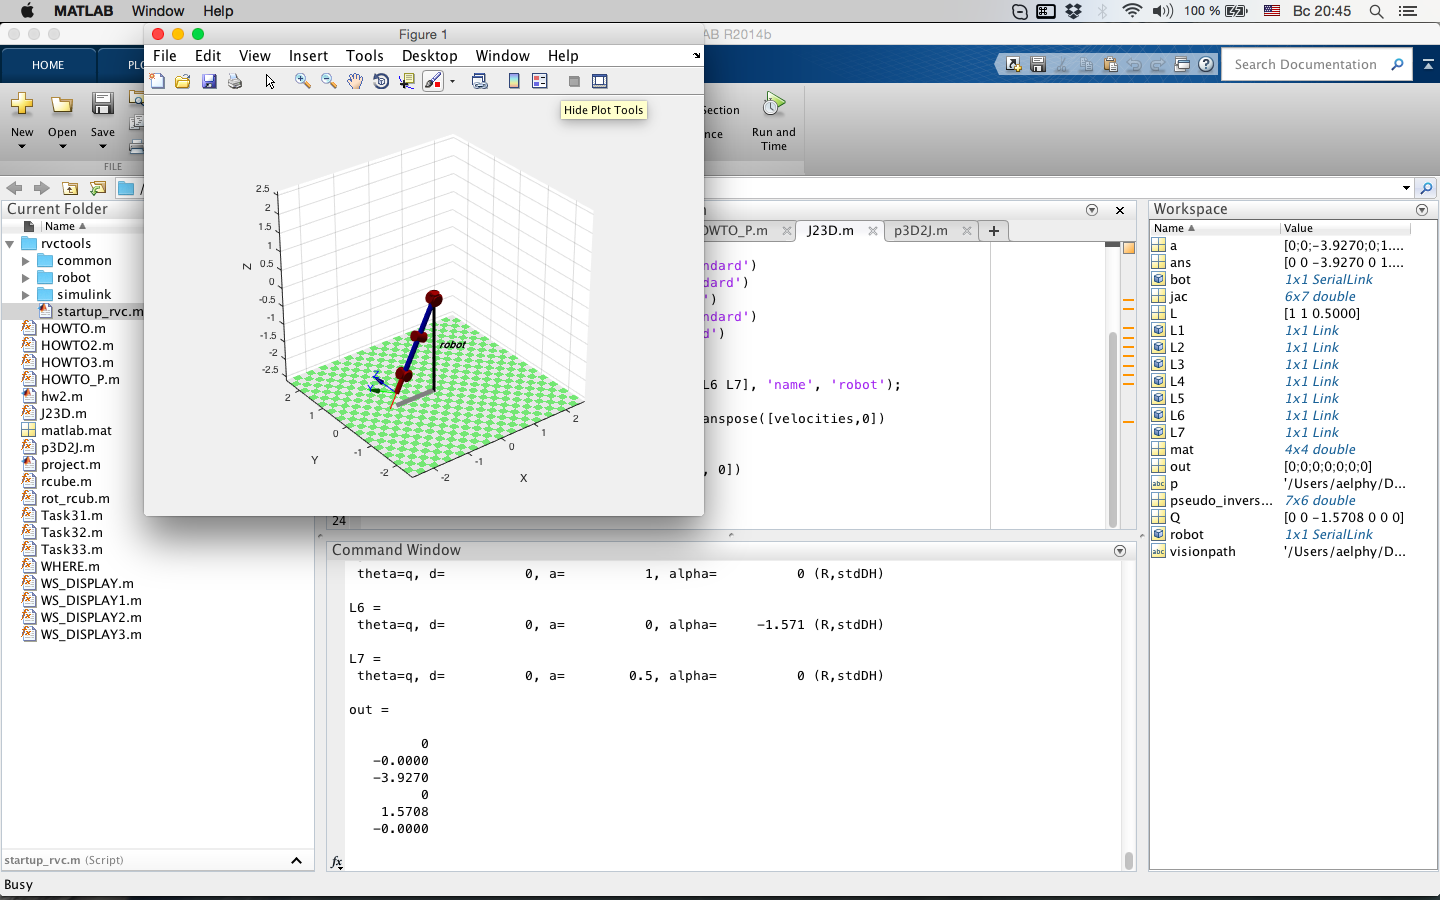
\includegraphics[width=15cm]{j23d}
\end{center}

3D2J - as input two vectors 3*3 - cartesian velocities.

\begin{center}
  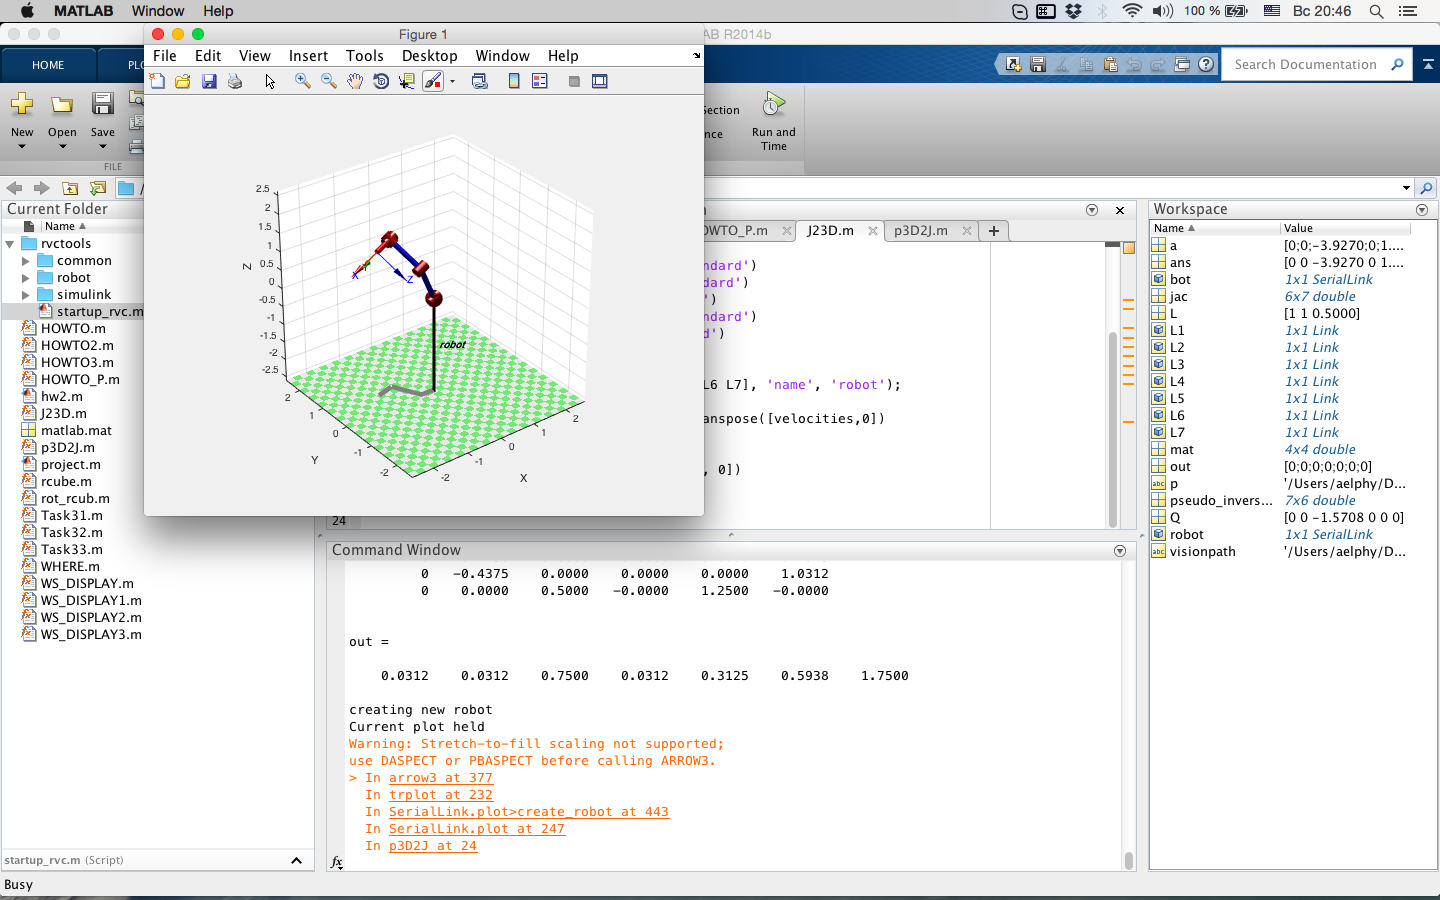
\includegraphics[width=15cm]{p3d2j}
\end{center}

\newpage

\begin{center}
\textbf{Appendix 2}
\end{center}

Commands:

project:

input - NULL, output - NULL
	
WHERE(Q):

input - [0         0   -1.5708         0         0         0]
	
output -
\[\left[
\begin{array}{cccc}
0 & -1 & 0 & 0 \\
0 & 0 & 1 & 0 \\
-1 & 0 & 0 & -2.5\\
0 & 0 & 0 & 1
\end{array} \right]\]
         			
WS\_DISPLAY:
	input - NULL, output - NULL
	
HOWTO\_P(ee\_matrix)

input: 
\[\left[
\begin{array}{cccc}
1 & 0 & 0 & 0 \\
0 & 0.6967 & -0.7174 & 0 \\
0 & 0.7174 & 0.6967 & 0\\
0 & 0 & 0 & 1
\end{array} \right]\]       
 
 output:       
 
 \[\left[
\begin{array}{cccc}
0.7827  & 0 & -0.6224  & 1.3063 \\
0.6224  & 0 & 0.7827 & 1.6007 \\
0 & -1 & 0 & 0\\
0 & 0 & 0 & 1
\end{array} \right]\]

J23D(velocities)

input: [0         0   -1.5708         0         0         0]

output: [0         0   -3.9270         0    1.5708         0]

\medskip

p3D2J(v\_velocities, w\_velocities)

input: [1,1,1], [1,1,1]

output: [0.0312    0.0312    0.7500    0.0312    0.3125    0.5938    1.7500]

\end{document}